\documentclass{article}

\usepackage{polski}
\usepackage{amsmath}
\usepackage{graphicx}
\usepackage{float}
\usepackage{subfig}
\usepackage{multirow}
\usepackage{chngpage}

\title{Przybliżanie funkcji - podsumowanie}
\author{\textbf{Łukasz Wala}\\
    \textit{AGH, Wydział Informatyki, Elektroniki i Telekomunikacji} \\
    \textit{Metody Obliczeniowe w Nauce i Technice 2021/2022}}
\date{Kraków, \today}

\begin{document}
\maketitle

\section{Wstęp}
W niniejszym podsumowaniu omówione zostaną zagadnienia przybliżania funkcji w odniesieniu do funkcji $f$.
Do użytych metod przybliżania należą:
\begin{itemize}
    \item
    interpolacja wegług metod Lagrange'a, Newtona oraz Hermite'a,
    \item
    interpolacja funkcjami sklejanymi,
    \item
    aproksymacja średniokwadratowa wielomianami algebraicznymi lub trygonometrycznymi.
\end{itemize}

Wszystkie te metody umożliwiają skonstruowanie funkcji przybliżającej na podstawie pewnej liczby punktów 
należących do funkcji $f$ przedstawionej wzorem:

\[f(x)=x^2-m\cdot\cos\left(\frac{\pi x}{k}\right)\]
Gdzie $k=\frac{1}{2}$, $m=4$ oraz $x\in [-6,6]$.

\section{Porównanie}
\subsection{Różnice}
Interpolacja zakłada, że skonstruowana funkcja będzie zawierała punkty, na podstawie których jest konstruowana.
Jest przydatna w np.:
\begin{itemize}
    \item
    zastępowaniu skomplikowanych funkcji np. wielomianami,
    \item
    całkowaniu numerycznym,
    \item
    znajdowaniu pochodnych w punktach pośrednich, rozwiązywaniu równań różniczkowych.
\end{itemize}

Aproksymacja średniokwadratowa nie ma natomiast podobnego założenia, co czyni ją ogólniejszą i pozwala zastosować, gdy
np. podane punkty zawierają błędy (wówczas interpolacja nie ma sensu), czy w przypadkach gdy warunek zawieranie punktów
po prostu nie jest konieczny.

\begin{figure}[H]
    \centering
    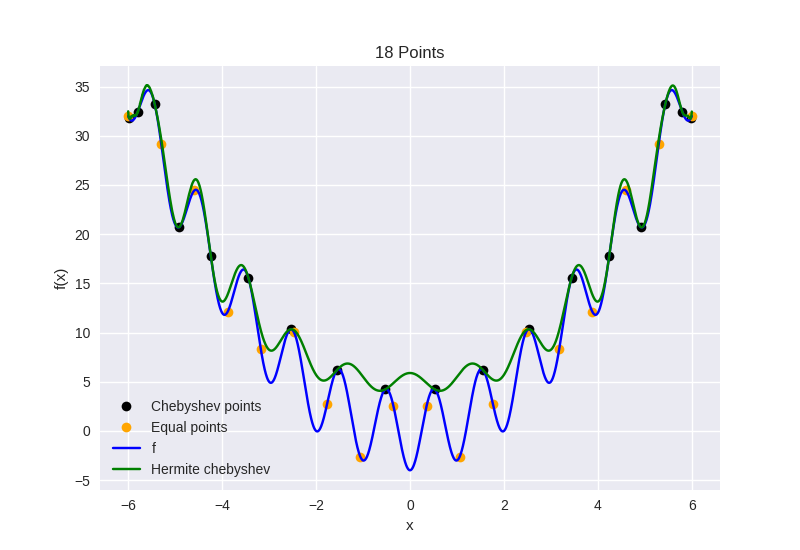
\includegraphics[width=\textwidth]{img/herm_18.png}
    \caption{Interpolacja - funkcja zawiera punkty}
\end{figure}

\begin{figure}[H]
    \centering
    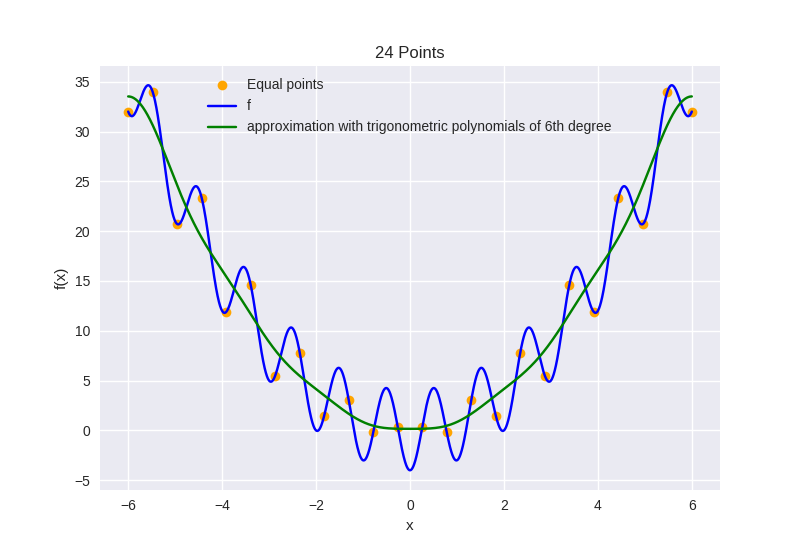
\includegraphics[width=\textwidth]{img/tripoly_6_24.png}
    \caption{Aproksymacja - funkcja nie musi zawierać punktów}
\end{figure}

Różnica pomiędzy metodami Lagrange'a a Newtona polega na sposobie konstrukcji wzoru. W metodzie Newtona dodanie nowego
węzła nie wiąże się z potwarzaniem obliczeń od początku, w metodzia Lagrange'a trzeba wykonywać mniej obliczeń podczas
wyznaczania wartości funkcji interplującej jak również łatwiej utworzyć wzór. W tym konkretnym przypadku
użycie metody Newtona wiązało się niestety z pojawieniem błędów numerycznych:

\begin{figure}[H]
    \centering
    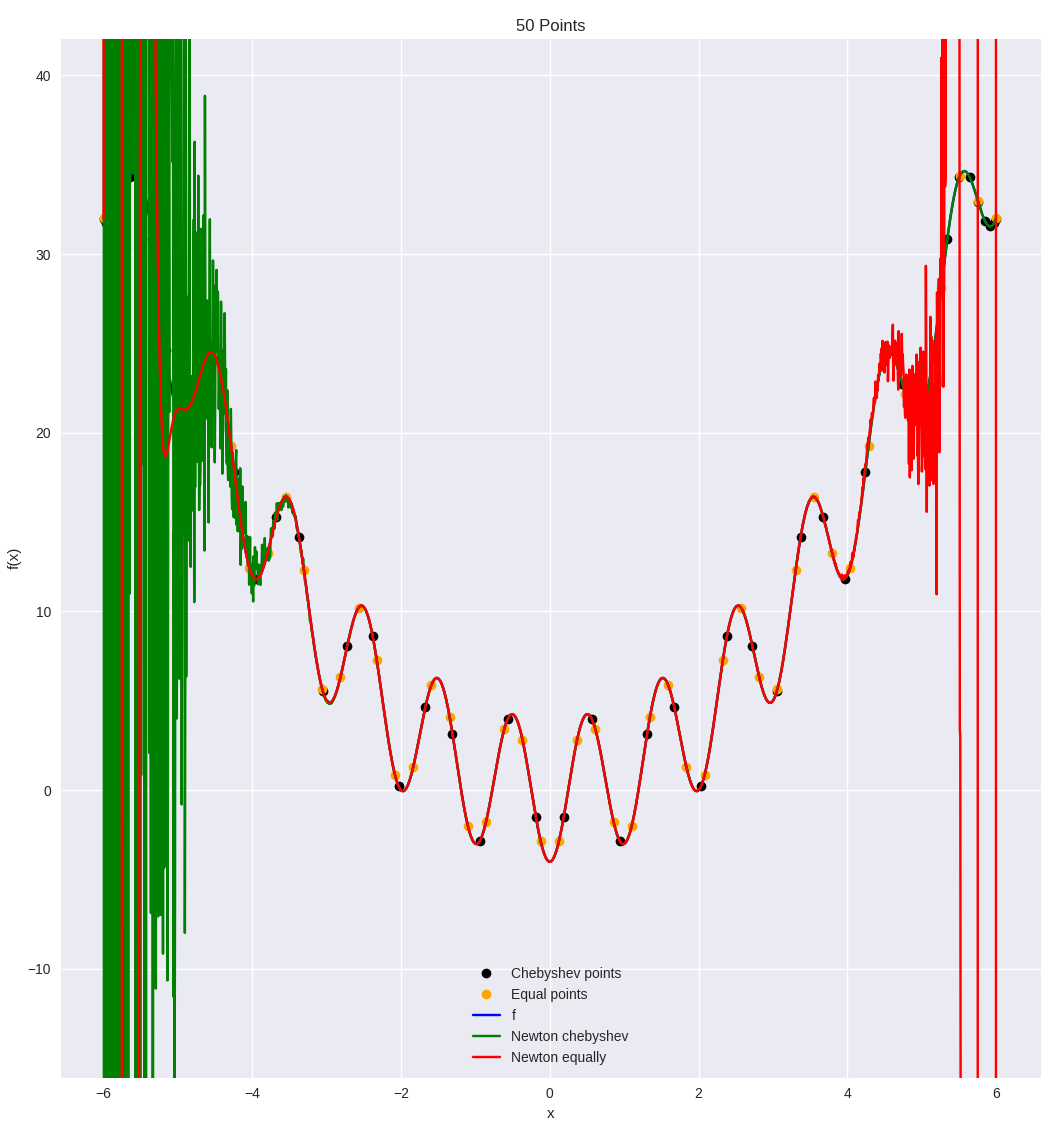
\includegraphics[width=\textwidth]{img/newt_50.png}
    \caption{Błedy numeryczne w metodzie Newtona}
\end{figure}

Podobny efekt wystąpił w metodzie Hermite'a, która jest bardzo podobna do metody Newtona, jednak pozwala również na zastosowanie
pochodnych w punktach.

\begin{figure}[H]
    \centering
    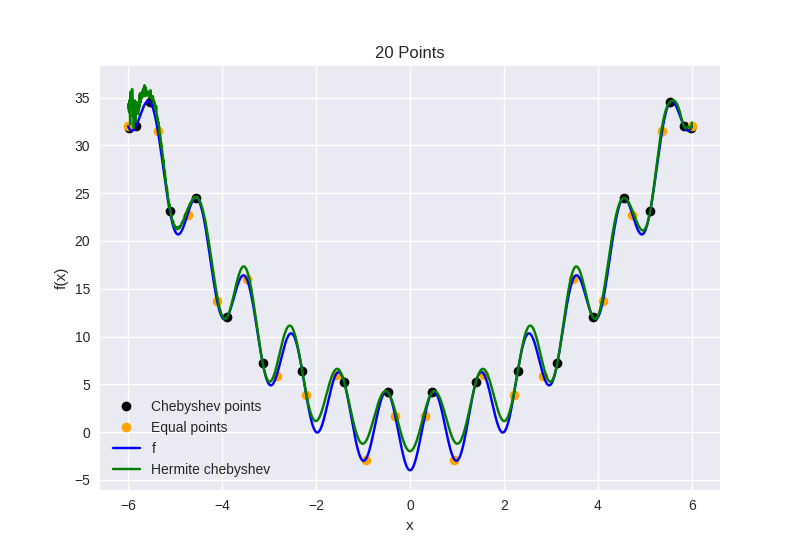
\includegraphics[width=\textwidth]{img/herm_20.png}
    \caption{Metoda Hermite'a - błędy numeryczne}
\end{figure}

Również w związku z tym, że funkcja musi zawierać wszystkie punkty na podstawie których jest tworzona, w metodach Newtona i 
Lagrange'a stopień wielomianu jest duży dla dużej liczby węzłów, co skutkuje problemami: 

\begin{figure}[H]
    \centering
    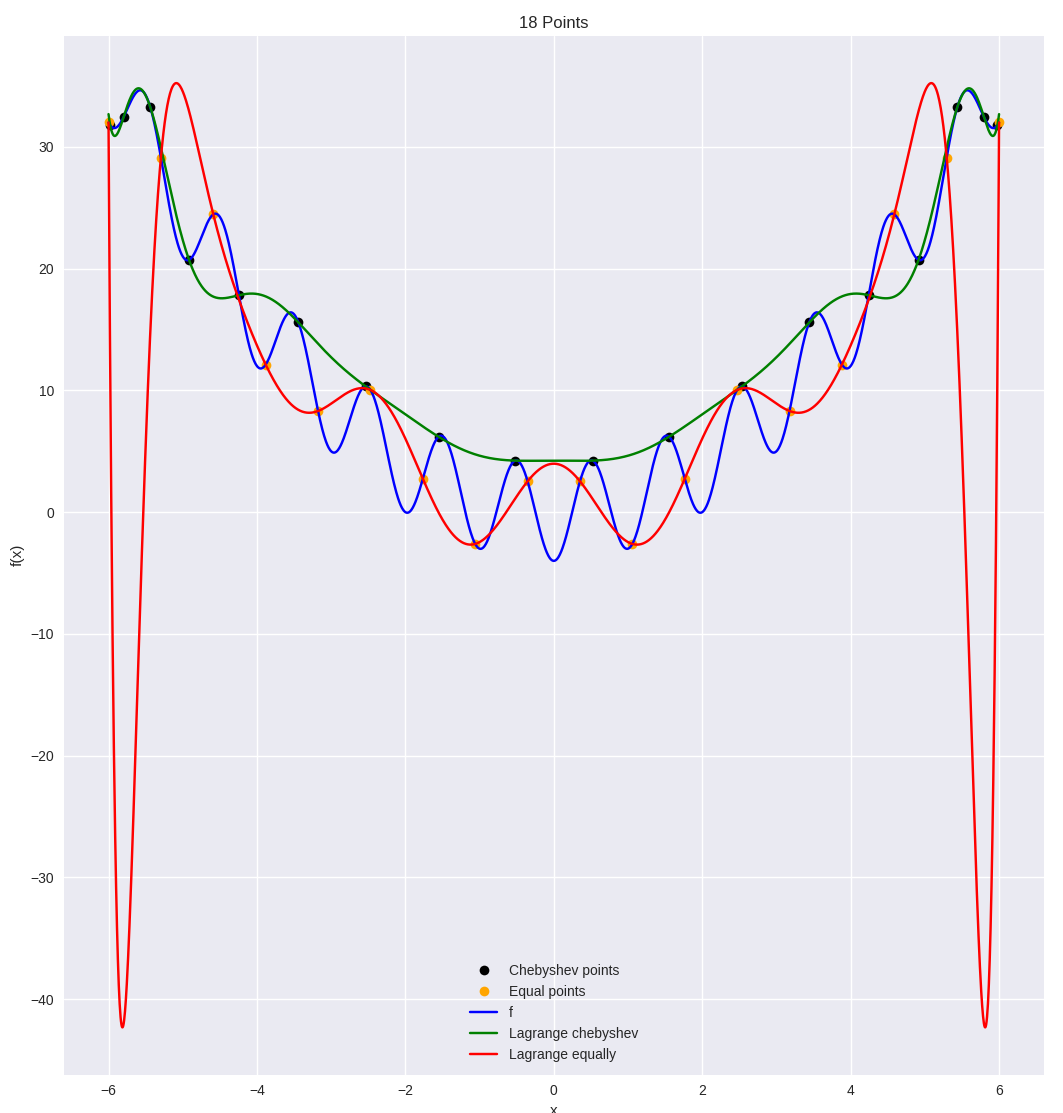
\includegraphics[width=\textwidth]{img/lagr_18.png}
    \caption{Efekt Rungego}
\end{figure}

Rozwiązaniem tego problemu jest zastosowanie specjalnego rozmieszczenia węzłów (według pierwiastków wielomianu Czebyszewa, na rysunku 4)
lub zastosowanie innej metody, jaką jest interpolacja funkcjami sklejanymi, która wykorzystuje wielomiany niskiego stopnia.

\begin{figure}[H]
    \centering
    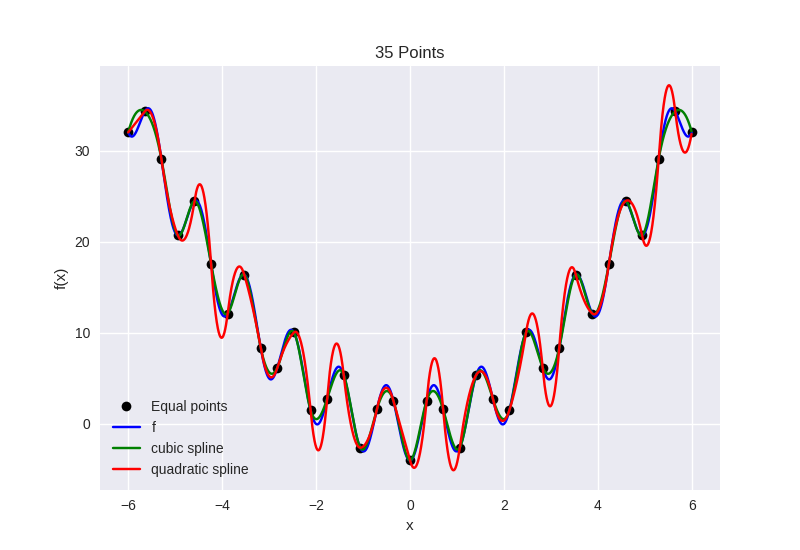
\includegraphics[width=\textwidth]{img/spline_35.png}
    \caption{Interpolacja splajnami}
\end{figure}

Interpolacja splajnami wymaga również podania warunków brzegowych. Zastosowany został warunek polegający na przybliżaniu trzecich
pochodnych ilorazami różnicowymi, inne badane warunki miały bardzo niewielki wpływ na funkcję przybliżającą.

Tutaj zastosowana została interpolacja funkcjami trzeciego stopnia, która jest najczęściej używana w praktyce, 
jednak można również stosować interpolację funkcjami sklejanymi np. drugiego
stopnia. Przy niej jednak niekiedy zdarzały się problemy jak oscylacja:

\begin{figure}[H]
    \centering
    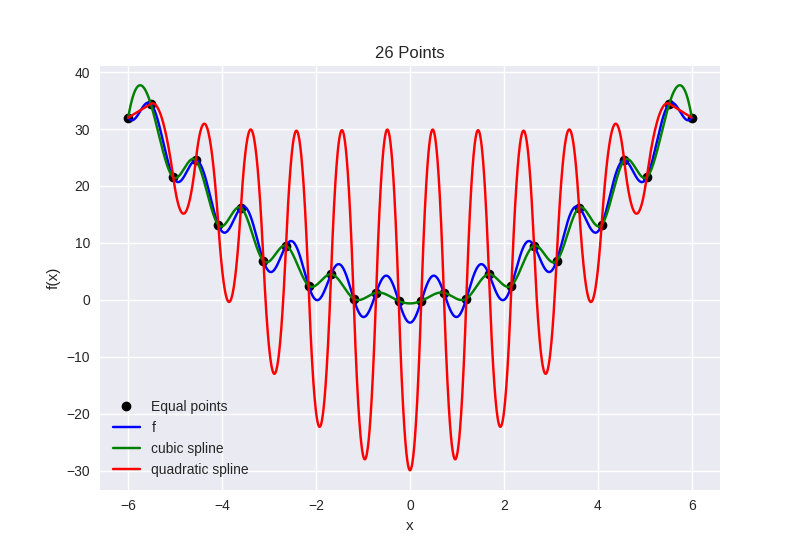
\includegraphics[width=\textwidth]{img/spline_26.png}
    \caption{Interpolacja splajnami drugiego stopnia - oscylacja}
\end{figure}

W przypadku aproksymacji średniokwadratowej, z racji tego, że punkty nie muszą należeć do funkcji, wybór stopnia wielomianu
jest dowolny, o ile liczba węzłów jest wystarczająca do jego skonstruowania:

\begin{figure}[H]
    \centering
    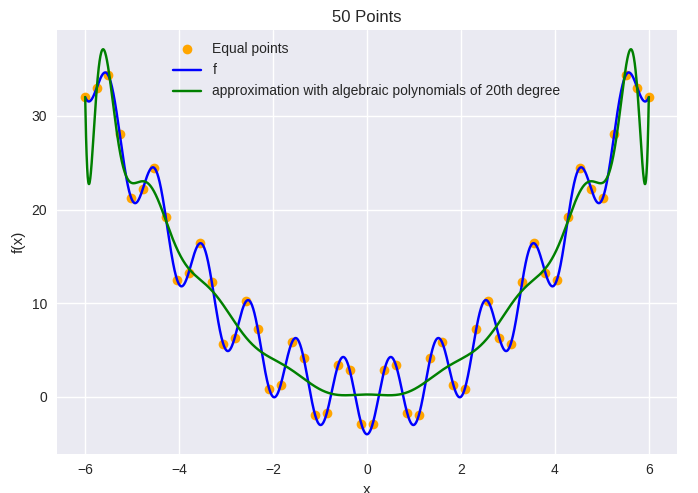
\includegraphics[width=\textwidth]{img/algpoly_20_50.png}
    \caption{Aproksymacja średniokwadratowa wielomianami algebraicznymi}
\end{figure}

Dla liczby węzłów dużo większej niż liczba funkcji bazowych zwykle następuje wygładzenie funkcji, np. jak na powyższym wykresie.

W aproksymacji średniokwadratowej wielomianami trygonometrycznymi stosowane są inne funkcje bazowe.
W tym konkretnym przypadku, ze względu na charakter funkcji $f$ sprawują się one lepiej pod względem dokładności:

\begin{figure}[H]
    \centering
    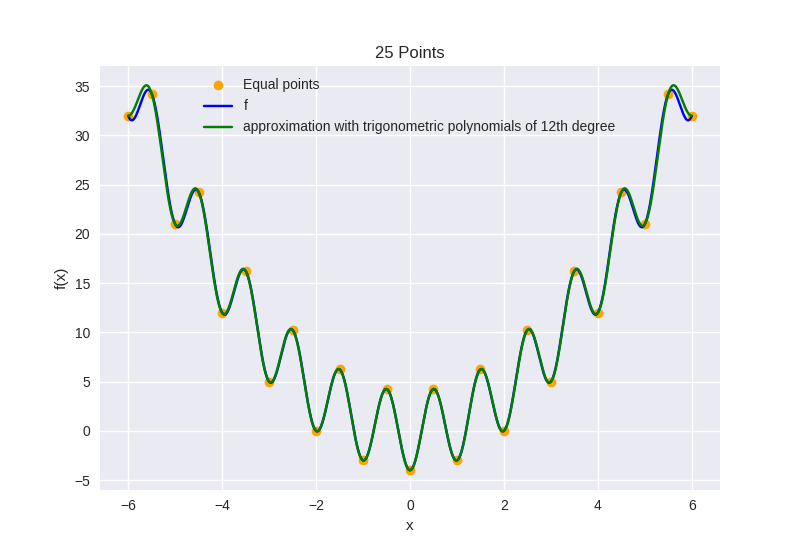
\includegraphics[width=\textwidth]{img/tripoly_12_25.png}
    \caption{Aproksymacja średniokwadratowa wielomianami trygonometrycznymi}
\end{figure}

\subsection{Dokładność}
Poniżej porównane zostaną dokładności dla różnych metod. Miarą dokładności będzie średnia kwadratów odległości funkcji $f$
oraz funkcji przybliżającej.

Metody interpolacji porónywane będą dla odpowiadających liczb informacji, czyli węzłów dla metod Lagrange'a, Newtona (rozmieszczenie Czebyszewa), 
węzłów oraz pierwszysch pochodnych dla metody Hermite'a, węzłów dla interpolacji splajnami trzeciego stopnia, 
węzłów dla aproksymacji, gdzie liczba funkcji bazowych odpowiada liczbie węzłów - 1 (w przypadku użycie liczby funkcji bazowych odpowiadających
liczbie węzłów wyniki byłby praktycznie jednoznaczne z interpolacją),
ponieważ to od liczby funkcji bazowych zależy rozmiar macierzy układu równań, wydaje się to być uczciwym porównaniem.

\begin{table}[H]
    \begin{tabular}{|l|l|l|l|l|l|l|}
    \hline
    \begin{tabular}[c]{@{}l@{}}Liczba\\ informacji\end{tabular} & Newton & Lagrange & Hermite & Splajny & Aprks. alg. & Aprks. tryg. \\ \hline
    4  &    12.862    &    12.862      &   1341.364      &  23.976       &    12.863         &    40.829          \\ \hline
    5  &  18.804      &   18.804       &    ...     &    23.976     &    9.280         &      ...        \\ \hline
    6  &  15.422      &   15.422       &    158.169     &   12.348      &   15.422          &    13.598          \\ \hline
    7  &   16.507     &   16.507       &     ...    &   23.976      &   11.933          &      ...        \\ \hline
    8  &   15.136     &    15.136      &  419.003       & 14.922        &   15.137          &   14.251           \\ \hline
    9  &   17.771     &   17.771       &    ...     &  16.951       &   17.843          &     ...         \\ \hline
    10 &   12.469     &  12.469        &  24.093       & 13.882        &    12.469         &   14.156           \\ \hline
    11 &  15.057      &   15.057       &    ...     &  15.939       &    12.363         &     ...         \\ \hline
    12 &   9.637     &   9.637       &   81.197      &  15.992       &   9.638          &   14.832           \\ \hline
    13 &  16.439      &  16.439        &   ...      &  23.976       &    15.182         &     ...         \\ \hline
    14 &  13.108      &   13.108       &  59.150       & 15.988        &   13.108          &  14.956            \\ \hline
    15 &  16.630      &  16.630        &    ...     &  15.993       &    16.710         &    ...          \\ \hline
    16 &   11.817     &   11.817       &  94.262       &  15.880       &   11.817          &  14.997            \\ \hline
    17 &  14.879      &  14.879       &     ...    &   15.449      &    14.857         &    ...          \\ \hline
    18 &  17.914      &   17.914       &   38.474      &  14.594       &   17.914          &  15.020            \\ \hline
    19 &  15.779      &   15.779       &    ...     &  13.364       &    16.662         &   ...           \\ \hline
    20 &  14.062      &    14.062      &   46.306      &  11.914       &    14.063         &  15.037            \\ \hline
    21 &  13.130      &    13.130      &   ...      &  10.403       &    13.213         &    ...          \\ \hline
    22 &  12.883     &    12.883      &  46.427       &  8.934       &    12.885         &   15.051           \\ \hline
    23 &  12.617      &   12.617       &    ...     &  7.549       &    12.882         &    ...          \\ \hline
    24 &  12.380      &   12.380       &   52.526      & 6.259        &   12.549          &   15.063           \\ \hline
    25 &  11.394      &   11.394       &    ...     &  1.081       &   11.611          &    ...          \\ \hline
    26 &  11.319      &   11.319       &   28.573      &  4.021       &   11.090          &   0.074           \\ \hline
    27 &  11.206      &   11.206       &    ...     &  3.117       &   10.877          &    ...          \\ \hline
    28 &  10.895      &  10.895        &  33.156       &  2.372       &   9.509          &    0.059          \\ \hline
    29 &  9.503      &   9.503       &    ...     &   1.778      &   9.884          &      ...        \\ \hline
    30 &  9.307      &    9.307      &  26.149       &  1.318       &   7.750          &    0.048          \\ \hline
    \end{tabular}
    \caption{Dokładności dla różnych metod}
\end{table}

Jak widać, interpolacja metodami Newtona, Lagrange'a oraz aproksymacja średniokwadratowa wielomianami algebraicznymi wykazują
prawie identyczne dokładność w badanym zakresie. Interpolacja metodą Hermite'a wykazuje mniejszą dokładność, jednak należy 
wziąć po uwagę, że wykorzystuje ona połowę mniej punktów w stosunku do innych metod, reszta informacji to pochodne w tych punktach.
Interpolacja splajnami cechuje się natomiast większą dokładnością, jak również nie używa wielomianów wysokich stopni, jak pozostałe
metody interpolacji. Najlepszą dokładność (ale tylko od pewnego momentu, tutaj 25 funkcji bazowych) ma funkcja stworzona przy pomocy
aproksymacji średniokwadratowej wielomianami trygonometrycznymi. 

\section{Wnioski}
Wszystkie przedstawione metody pozwalają, z pewnymi ograniczeniami, skutecznie przybliżyć funkcję $f$, jednak niektóre robią to lepiej,
lub mogą zostać zastosowane w szczególnych przypadkach, np. gdy funkcja przybliżająca musi zawierać wszystkie punkty, na podstawie
których jest konstruowana, najlepiej zastosować interpolację funkcjami sklejanymi. Gdy dostępne są również pochodne w punktach, 
zastosować można metodę Hermite'a. Jeżeli funkcja nie musi spełniać warunku zawierania punktów, dużo dokładność można uzyskać za
pomocą aproksymaji średniokwadratowej wielomianami trygonometrycznymi. Każda z metod posiada również pewne wady, np. błędy numeryczne
dla dużych liczb węzłów w metodzie Hermite'a, stąd metoda musi być odpowiednio dobrana do potrzeb.

\end{document}